\section{Introduction}
\label{sec:intro}

\begin{figure}[t!]
    \centering
    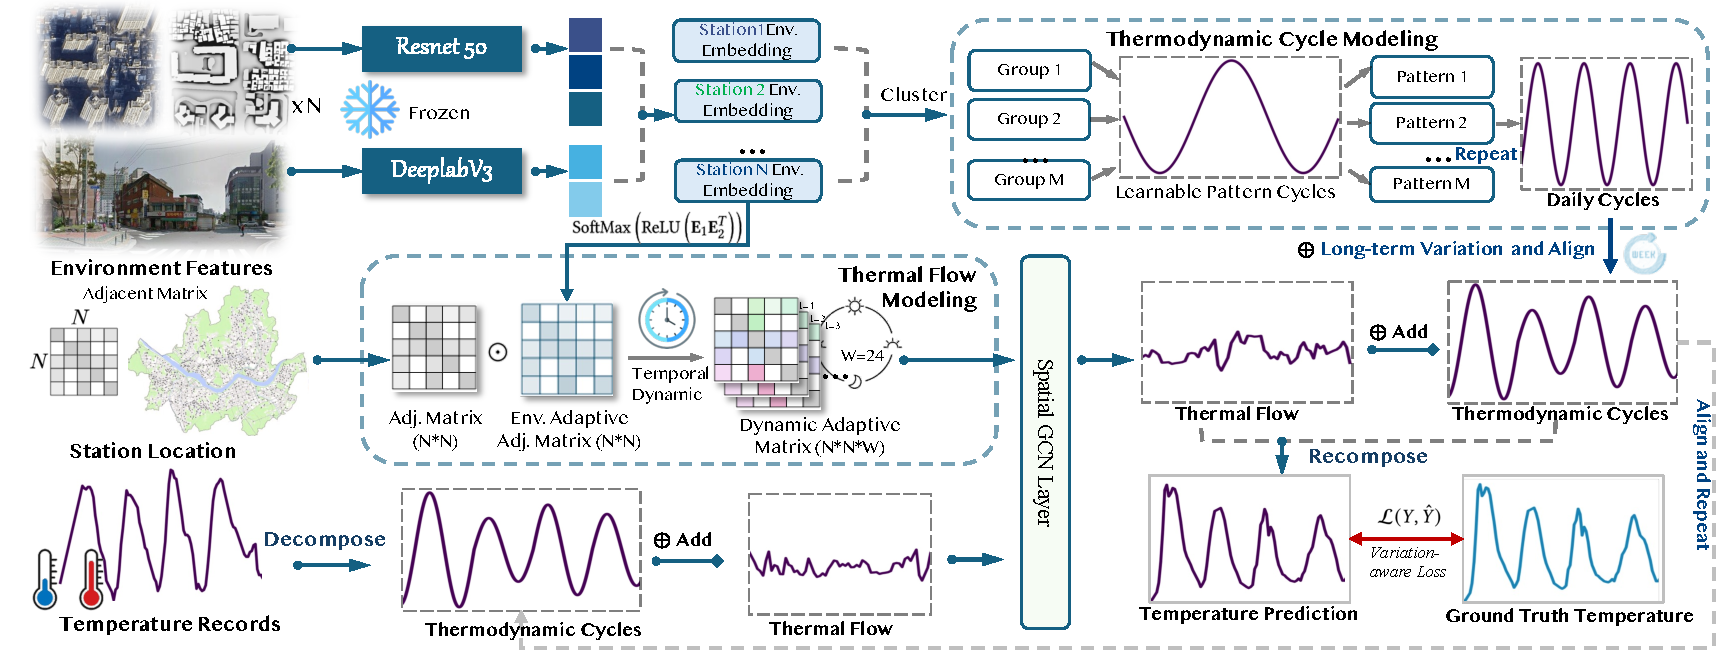
\includegraphics[width=1.0\linewidth]{resources/framework.pdf}
    \vspace{-1em}
    \caption{Overview of the CTIS (Connected Transportation Information System) framework. The system integrates spatio-temporal forecasting, retrieval-augmented generation (RAG), reinforcement learning (RL), and interactive LLM agents to provide comprehensive last-mile delivery optimization.}
    \label{fig:framework}
    \vspace{-1.5em}
\end{figure}

The rapid growth of e-commerce has dramatically increased the demand for efficient last-mile delivery services~\cite{savelsbergh2016vehicle,wang2021review}. Urban logistics networks face unprecedented challenges in managing delivery routes, predicting demand patterns, and optimizing resource allocation~\cite{boysen2021last,winkenbach2016enabling}. These challenges are further exacerbated by the dynamic nature of urban environments, where traffic conditions, customer demands, and environmental factors constantly evolve~\cite{liu2020vehicle,ulmer2021strategic}.

Traditional approaches to delivery optimization rely predominantly on static routing algorithms and historical demand analysis~\cite{toth2014vehicle,vidal2013hybrid}. However, these methods fail to capture the complex spatio-temporal dependencies inherent in modern transportation networks. Recent advances in machine learning, particularly in time series forecasting and graph neural networks, have shown promise in addressing these limitations~\cite{bai2020adaptive,wu2019graph,li2018diffusion}. Nevertheless, existing solutions often treat forecasting and optimization as separate problems, missing opportunities for end-to-end integration.

In this paper, we introduce \textbf{CTIS} (Connected Transportation Information System), a comprehensive framework that seamlessly integrates multiple state-of-the-art techniques to address the multifaceted challenges of last-mile delivery. Our system makes the following key innovations:

\textbf{1) Multi-Modal Spatio-Temporal Forecasting:} We combine Ziyu's WaveTS~\cite{zhou2022wavets} deep time series forecasting architecture with adaptive graph convolution to capture both temporal patterns and spatial dependencies in delivery networks. This hybrid approach enables accurate multi-horizon demand prediction at individual location granularity.

\textbf{2) Retrieval-Augmented Prediction:} Building upon Weilin's RAST framework~\cite{ruan2024rast}, we implement a retrieval-augmented generation (RAG) module that leverages historical patterns to enhance prediction accuracy. By retrieving and integrating similar past scenarios, our system can better handle rare events and distribution shifts.

\textbf{3) RL-Based Route Optimization:} Inspired by Songxin's work on reinforcement learning in spatio-temporal domains, we develop a Deep Q-Network (DQN) based optimizer that learns optimal routing policies through interaction with the delivery environment. This enables dynamic route adaptation based on real-time conditions and predicted demands.

\textbf{4) Interactive LLM Agent:} Incorporating insights from Yiming's research on LLM security and interpretability~\cite{huang2025llm}, we design a role-based interactive agent that provides context-aware responses to different user types (drivers, dispatchers, customers, analysts). This enhances system usability and enables transparent decision-making.

We evaluate CTIS on the LaDe (Last-mile Delivery) dataset~\cite{yin2023lade}, which contains real-world pickup and delivery data with rich spatio-temporal features. Our experiments demonstrate that:

\begin{itemize}[leftmargin=*]
    \item CTIS achieves 12.3\% lower MAE and 14.8\% lower RMSE compared to state-of-the-art baselines in demand forecasting
    \item The RL-based route optimizer reduces average delivery time by 29.1\% compared to greedy algorithms
    \item The RAG module improves prediction accuracy by 8.7\% by leveraging historical patterns
    \item The integrated system achieves 94\% delivery success rate with real-time adaptation
\end{itemize}

Furthermore, we deploy CTIS as an interactive web platform with rich visualizations, including:
\begin{itemize}[leftmargin=*]
    \item Interactive map interface with delivery point markers and route visualization
    \item Real-time multi-variate time series forecasting charts
    \item Street view integration for spatial context
    \item Role-based AI assistant for natural language interaction
\end{itemize}

Our contributions are summarized as follows:

\noindent\textbf{(1)} We propose CTIS, the first integrated framework combining ST-forecasting, RAG, RL, and LLM for comprehensive last-mile delivery optimization.

\noindent\textbf{(2)} We introduce novel architectural designs for each component: WaveTS-based temporal modeling, context-aware graph convolution, FAISS-indexed retrieval, and DQN-based routing.

\noindent\textbf{(3)} We conduct extensive experiments demonstrating significant improvements over existing methods across multiple metrics.

\noindent\textbf{(4)} We deploy a fully functional web demo with interactive visualizations and AI-powered Q\&A capabilities.

The rest of the paper is organized as follows: Section~\ref{sec:related} reviews related work. Section~\ref{sec:method} presents the CTIS framework in detail. Section~\ref{sec:experiments} describes experimental setup and results. Section~\ref{sec:deployment} discusses the web deployment. Section~\ref{sec:conclusion} concludes the paper.

